\chapter{La rivoluzione di AlphaFold}

Predire la struttura delle proteine è stato un importante problema di ricerca, aperto per più di 50 anni. Nonostante i vari progressi, nessun metodo è riuscito ad arrivare ad una precisione atomica, specialmente nel caso in cui non siano disponibili delle proteine omologhe. AlphaFold2 è il primo metodo computazionale che può regolarmente predire la struttura delle proteine con accuratezza atomica, anche in casi in cui nessuna struttura simile è conosciuta\supercite{jumper2021highly}.
AlphaFold2 (AF2) è la versione interamente ridisegnata del modello basato su reti neurali AlphaFold, entrambi sviluppati da DeepMind. 

\par Nel CASP14 (2020) AF2 viene dichiarato vincitore del "protein structure prediction problem" per la maggior parte delle proteine a 1 dominio, dimostrando accuratezza competitiva con le strutture sperimentali nella maggioranza dei casi e superando di gran lunga tutti gli altri metodi esistenti. Alla base di AF2 c'è un nuovo approccio basato sul Machine Learning, che unisce nel design dell'algoritmo di deep learning conoscenza fisica e biologica sulla struttura delle proteine, facendo leva sugli allineamenti multi-sequenza.

\par Quando è iniziata a circolare la notizia che AF2 avesse risolto il problema del PSP, si pensava che avesse raggiunto un GDT\_TS medio di 80 \supercite{moalqAF2} (intuitivamente significa che in media l'80\% della struttura delle proteine target fosse stato predetto). Predizioni casuali forniscono un GDT $\leq 20 \%$, predire la struttura grossolanamente è associato a un GDT\_TS di circa il 50\% mentre predire una topologia accurata porta con sè un valore di circa il 70\%. Quando tutti i dettagli, comprese le conformazioni delle side-chain, sono corretti il GDT\_TS supera il 90\%. Alcuni, tra cui Mohammed AlQuraishi\footnote{Assistant Professor, Department of Systems Biology della Columbia University e principale investigatore dell'Alquraishi Laboratory. È stato anche uno dei peer reviewer del paper di AlphaFold2\supercite{moalqAF2}.} suggerivano che ci sarebbero voluti almeno altri 10 anni per arrivare ad un GDT di 85-90\supercite{moAlq}, ma AlphaFold ha riportato una mediana di GDT\_TS pari a 92.4. Un valore che AlQuraishi definisce come uno degli avanzamenti scientifici più rapidi degli ultimi decenni.

\par Le strutture di AF2 hanno un'accuratezza riguardo la mediana della backbone\footnote{La notazione indica C$_{\alpha}$ mean root square deviation ad una copertura del 95\% dei residui. L'intervallo con 95\% di confidenza riportato in questo caso da AF2 corrisponde a 0.85-1.16 \angstrom.} di 0.96 RMSD$_{95}$, mentre il prossimo miglior metodo ha dimostrato un'accuratezza di 2.8 \angstrom. In figura \ref{fig:z-score} è possibile vedere il confronto dei vari metodi che hanno partecipato al CASP14 valutati secondo il Z-score\footnote{Lo Z-score è la differenza del valore di un campione rispetto alla media della popolazione, divisa per la deviazione standard; un valore alto rappresenta una grande deviazione dalla media ed è comunemente usato come procedura di rilevamento dei valori anomali.}. 

\begin{figure}[!htb]
	\centering
	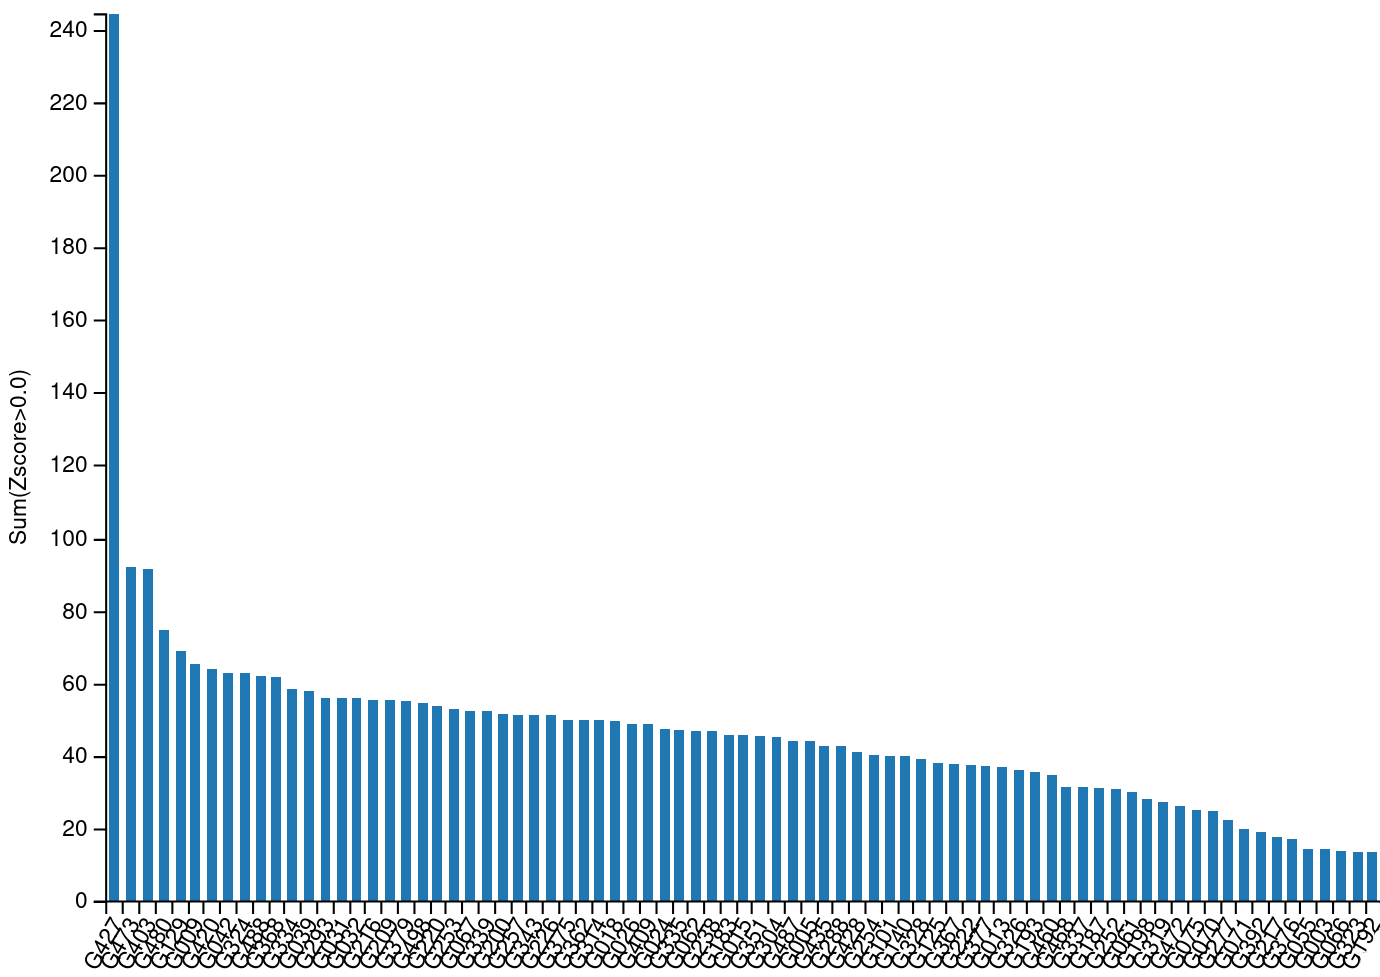
\includegraphics[scale=0.45]{images/casp_res.png}
	\caption{Risultati del CASP14 in base al Z-score. AlphaFold (G427) è incredibilmente avanti rispetto al secondo gruppo (473, Baker). Fonte\cite{CaspRes}}
	\label{fig:z-score}
\end{figure}

Per quanto riguarda l'accuratezza non solo della backbone ma di tutti gli atomi, AlphaFold ha registrato un'accuratezza di 1.5 \angstrom (per fare un confronto, un atomo di carbonio è largo approssimativamente 1.4 \angstrom).

\begin{figure}[!htb]
	\minipage{0.5\textwidth}
	\centering
	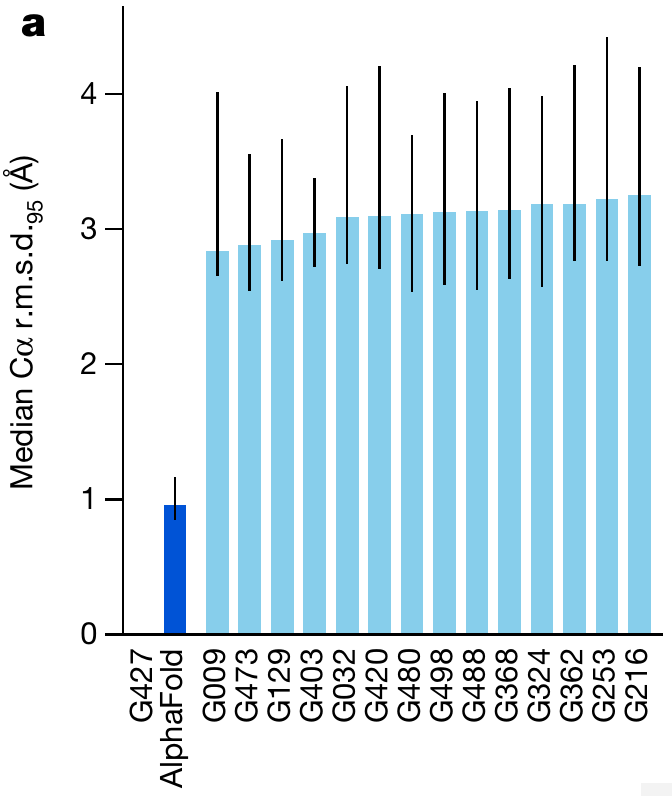
\includegraphics[scale=0.3]{images/af-res.png}
	\caption{Performance di AF2 sul dataset del CASP14 (n=87 domini di proteine) rispetto agli altri migliori 15 metodi (su 146). Fonte\cite{jumper2021highly}}
	\label{fig:performanceAF2}
	\endminipage\hfill
	\minipage{0.48\textwidth}
	\centering
	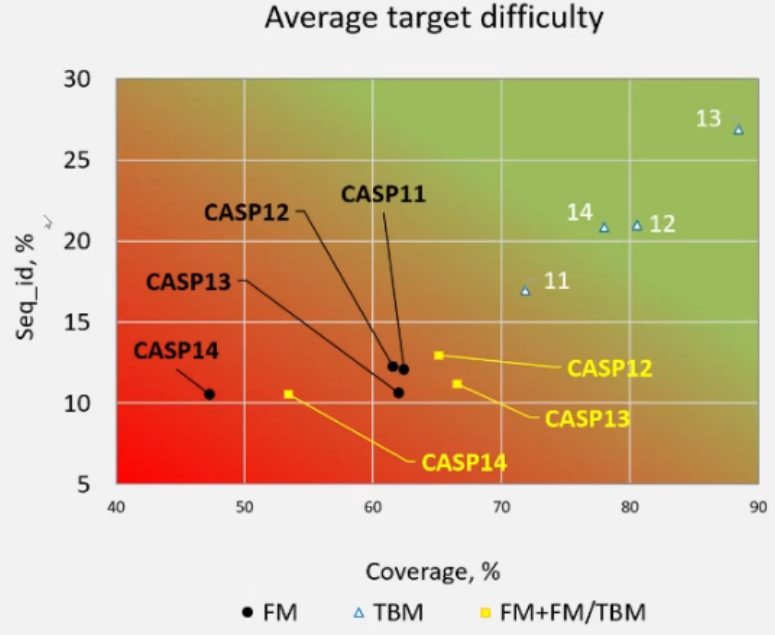
\includegraphics[scale=0.3]{images/casp-difficuty.png}
	\caption{Confronto degli obiettivi degli ultimi quattro CASP in termini di copertura e identità di sequenza dei modelli disponibili. In entrambi i casi, CASP14 include gli obiettivi di modellazione libera (FM) più difficili mai forniti. Fonte\cite{blopigAF}}
	\label{fig:casp-difficulty}
	\endminipage\hfill
\end{figure}

In alcuni casi le predizioni di AlphFold erano talmente accurate da superare i risultati sperimentali facendo mettere in discussione agli sperimentatori i risultati da loro ottenuti. Si potrebbe pensare che i target del CASP14 fossero in qualche misura più semplici rispetto a quelli degli altri anni per spiegare il successo di AlphaFold. Ma non è così, anzi, gli organizzatori hanno dimostrato che è stato il CASP più difficile (in quanto a percentuale di identità di sequenze).

Un esempio in cui AF2 surclassa gli altri metodi è il target T1064. AF2 riesce ad ottenere una similitudine molto alta, con nucleo e strutture secondarie quasi perfette (nonostante una grande regione di loop sia sbagliata, ma questo potrebbe anche indicare che sia una regione flessibile).

\begin{figure}[!htb]
	\minipage{0.48\textwidth}
	\centering
	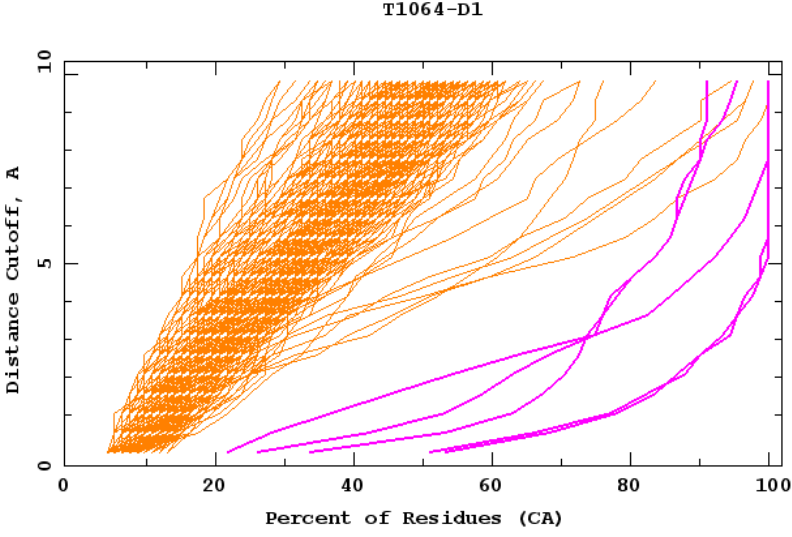
\includegraphics[scale=0.3]{images/t1064-af2.png}
	\caption{Analisi GDT dei 508 modelli inviati per la sequenza target T1064-D1. L'analisi denota il più grande insieme di atomi di $C_{\alpha}$ (percentuale della struttura modellata) che può rientrare nella distanza cutoff $ \in \{ 0.5 \angstrom, 1.0 \angstrom, 1.5 \angstrom, ... , 10.0 \angstrom \} $. In viola i modelli di AlphaFold. Fonte: \cite{CaspRes}}
	\label{fig:t1064-chart}
	\endminipage\hfill
	\minipage{0.5\textwidth}
	\centering
	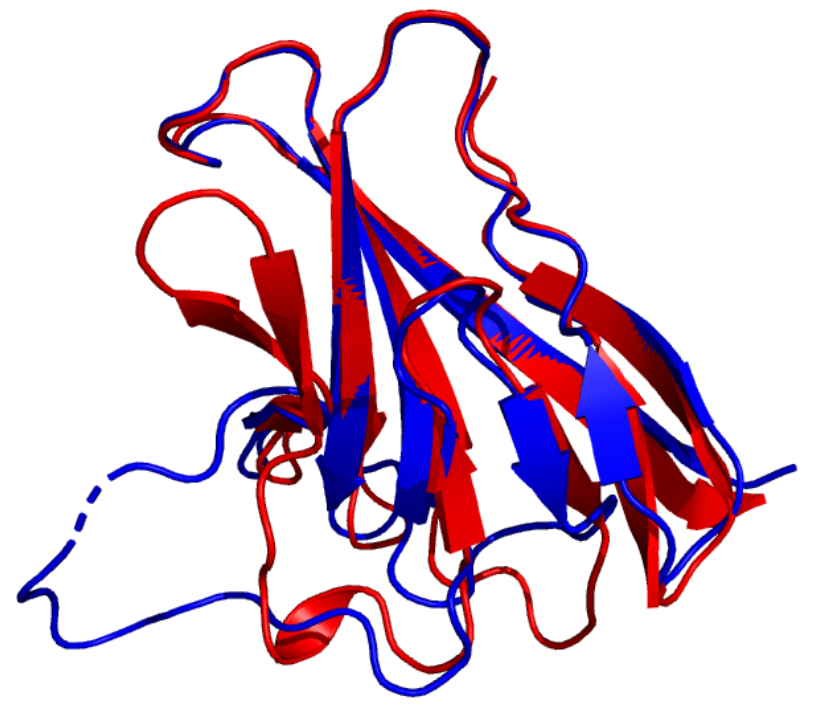
\includegraphics[scale=0.3]{images/t1064_model.png}
	\caption{(rosso) modello di AF2 per il target T1064. (blu) struttura 7JTL\_A. Fonte \cite{blopigAF}}
	\label{fig:t1064-afmodel}
	\endminipage\hfill
\end{figure}

Gli altri metodi predicono questa struttura in modo nettamente peggiore. Prendendo in considerazione i risultati dei gruppi Baker e Zhang (i due migliori subito dopo AF2, basati prevalentemente sulla pipeline del primo AlphaFold)  si può notare che il nucleo della proteina è totalmente sbagliato e ci sono molte differenze con la struttura sperimentale (vedi fig. \ref{fig:altri-modelli-t1064}).

\begin{figure}[!htb]
	\centering
	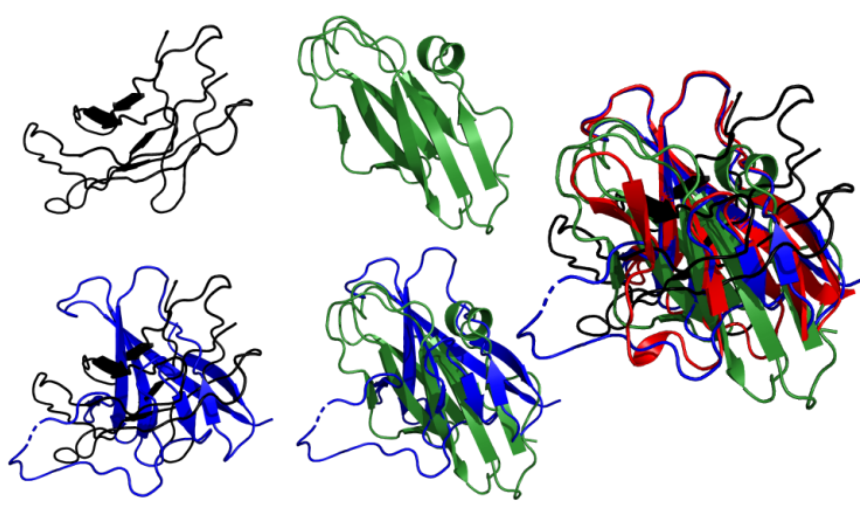
\includegraphics[scale=0.7]{images/t1064-altri-modelli.png}
	\caption{Modelli con il punteggio più alto per il target T1064 presentati dai gruppi Zhang (nero) e Baker (verde). In basso: modelli allineati con la struttura cristallina. A destra: tutti e tre i modelli (Zhang, Baker e AlphaFold 2) sono allineati con la struttura cristallina. Fonte\cite{blopigAF}}
	\label{fig:altri-modelli-t1064}
\end{figure}

Come è possibile vedere nel grafico in figura \ref{fig:modelli-casp14} AF2 vince quasi in tutti i target, ci sono addirittura casi in cui il prossimo miglior metodo raggiunge solo il 20\% dell'accuratezza mentre AF è al 90\%.

\begin{figure}[!htb]
	\centering
	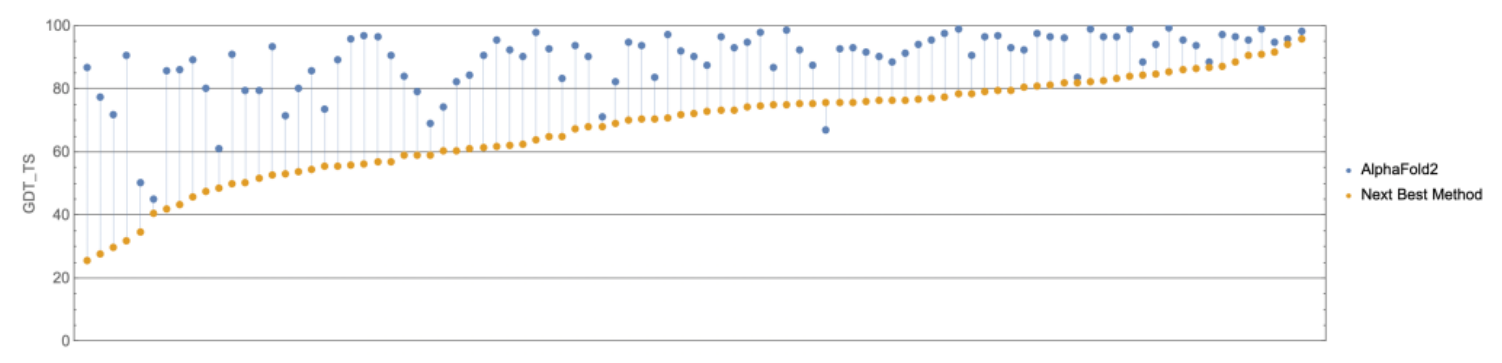
\includegraphics[scale=0.4]{images/models1.png}
	\caption{Il grafico mostra la differenza fra AF2 e il prossimo miglior metodo in tutti i target del CASP14. Fonte\cite{moAlq}}
	\label{fig:modelli-casp14}
\end{figure}

In generale, anche quando gli altri modelli predicono bene, è nei dettagli che AF2 si differenzia e porta la predizione ad un livello superiore (vedi fig. \ref{fig:af2-details}).

\begin{figure}[!htb]
	\centering
	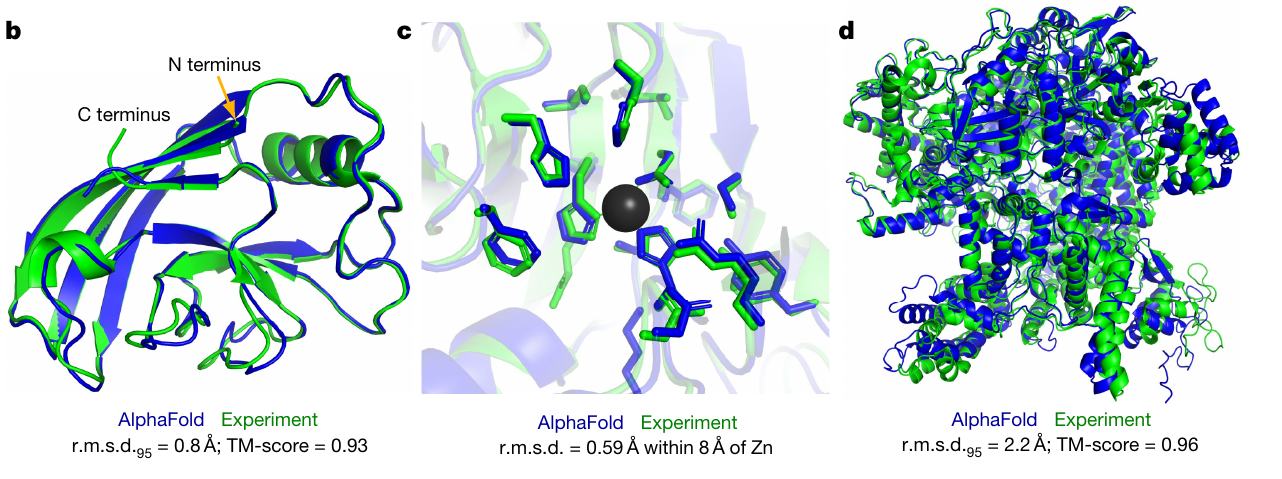
\includegraphics[scale=0.5]{images/af2-details.png}
	\caption{Predizioni di AF2 (in blu) sovrapposte alle strutture sperimentali (in verde) sui target: T1049, T1056, T1044. In (c) è possibile notare una corretta predizione di un sito di legame per lo zinco. La struttura in (d) è composta da 2180 residui. Fonte\cite{jumper2021highly}}
	\label{fig:af2-details}
\end{figure}

\par AlphaFold2 è in grado di fornire delle precise stime della sua affidabilità per residuo in modo da consentire un uso consapevole delle sue predizioni. La sua misura di confidenza (pLDDT) predice affidabilmente l'accuratezza lDDT-C$_{\alpha}$ della predizione corrispondente. AF2 si è dimostrato applicabile anche su proteine molto lunghe. 

\par La rivoluzione di AlphaFold è stata assimilata alla rivoluzione avvenuta nell'ImageNet nel 2012. Ma secondo AlQuraishi le due cose non sono paragonabili. In quell'occasione il deep learning ha dimostrato di poter superare gli approcci convenzionali nel riconoscimento delle immagini sconvolgendo il mondo della computer vision. Rispetto all'avanzamento di AF2 vi è però una differenza importante: l'avanzamento di ImageNet è stato incrementale, quello di AF2 è invece un balzo in avanti di 10 anni, un cambiamento così profondo da mettere sottosopra un intero campo nel corso di una notte; è stato come avere l'accuratezza nell' ImageNet del 2020 già nel 2012, senza tutti i passi intermedi.

\subsubsection{Utilizzo di AF2}

Il codice sorgente di AlphaFold è stato reso pubblico da DeepMind ed è disponibile su GitHub\footnote{https://github.com/deepmind/alphafold}. Per funzionare AlphaFold ha bisogno di database di supporto (fino a 2.5 TB), di molta memoria e di potenza computazionale. Per questi motivi è verosimile utilizzarlo solo su server dedicati alla computazione, come quello disponibile all'Università di Pisa.

\par Il codice è rilasciato con un'immagine Docker e un \textit{launcher script} associato, in modo da risultare più facilmente accessibile. 

\par È stata anche pubblicata una versione semplificata di AlphaFold (senza uso di template) tramite un Google Colab notebook\footnote{https://colab.research.google.com/github/deepmind/alphafold/blob/main/notebooks/AlphaFold.ipynb}.


\section{Architettura}

Forse l'osservazione più importante da fare su AlphaFold è che DeepMind \textit{non} ha scoperto nessun nuovo e sbalorditivo principio sul protein folding. Non ci sono sorprese di carattere biologico. Tutto si basa su un ottimo design del sistema di DL e sul livello altissimo delle abilità dei membri del team e delle risorse a disposizione. È possibile porsi domande sul perché la struttura sia proprio come è presentata nel paper. La risposta più probabile risiede nell'intensa sperimentazione, attuata grazie ad una grande quantità di risorse computazionali e guidata da una grande capacità di progettazione del team di DeepMind.

\par Uno dei principi su cui si basa AlphaFold è l'immersione delle intuizioni basate sulla conoscenza fisico-chimica delle proteine direttamente nella struttura della rete, non come un processo intorno ad essa. Il bias induttivo del sistema riflette la conoscenza attuale fisica e geometrica delle proteine, sminuendo l'importanza della posizione dei residui nella sequenza ed enfatizzando invece la comunicazione tra i residui vicini nella proteina ripiegata. La rete apprende iterativamente un grafo delle interazioni fra residui, ragionando su questo grafo implicito mentre viene costruito. AlphaFold è un sistema end-to-end che produce direttamente una struttura invece di fornire come output le distanze inter-residuo.

\begin{figure}[!htb]
	\centering
	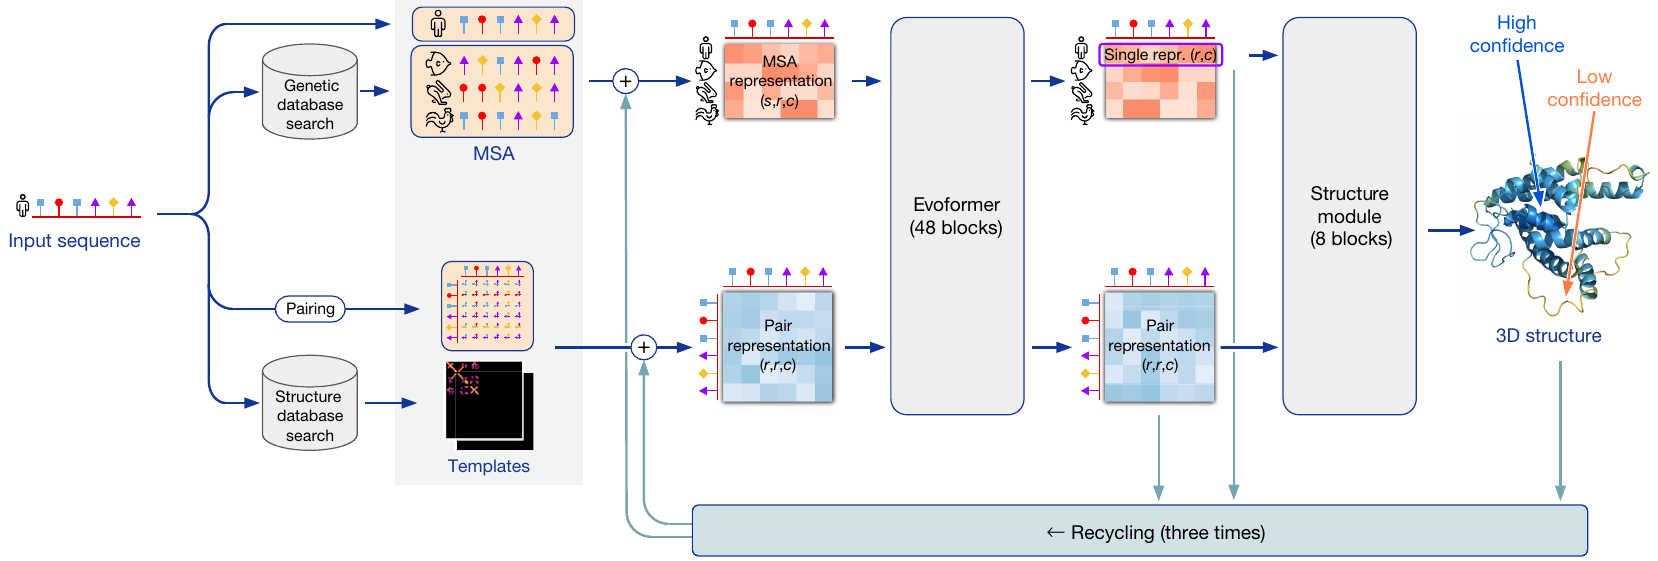
\includegraphics[scale=0.38]{images/af-archit.png}
	\caption{Schema architetturale di AF2. Le frecce indicano il flusso dell'informazione. Le dimensioni degli array sono riportate fra parentesi (s=numero di sequenze, r=numero di residui, c=numero di canali). Fonte\cite{jumper2021highly}}
	\label{fig:architettura-af2}
\end{figure}

L'architettura principale di AlphaFold può essere suddivisa in 3 componenti principali. Innanzitutto vi è la parte di \textit{preprocessing} dell'input, dove AF2 utilizza la sequenza di amminoacidi in ingresso per interrogare diversi database di sequenze proteiche e costruisce un MSA e quindi una \textit{MSA representation}. AlphaFold 2 cerca anche di identificare le proteine che possono avere una struttura simile all'input (template) e costruisce una rappresentazione iniziale dei contatti nella struttura, chiamata \textit{pair representation}. Questo è, in sostanza, un modello di quali amminoacidi è probabile siano in contatto tra loro. La prima parte della struttura di AF2 non aggiunge niente di rivoluzionario alla pipeline dei sistemi di predizione. Vengono utilizzati anche database di metagenomica\footnote{L'applicazione di moderne tecniche di genomica senza la necessità di isolare e coltivare in laboratorio specie singole, studiandole quindi direttamente nel loro ambiente naturale.} come MGnify.

\par Nella seconda parte del diagramma, AlphaFold 2 prende l'MSA e i template e li passa attraverso un \textit{transformer} (lo si può, per ora, immaginare come un "oracolo" in grado di identificare rapidamente quali informazioni siano più informative). L'obiettivo di questa parte è perfezionare le rappresentazioni sia per l'MSA che per le interazioni di coppia, anche scambiando informazioni tra loro in modo iterativo. Un modello migliore dell'MSA migliorerà la caratterizzazione della geometria della rete, che contemporaneamente aiuterà a perfezionare il modello dell'MSA. Questo processo è organizzato in blocchi che vengono ripetuti in modo iterativo fino a un numero specificato di cicli (48 blocchi nel modello pubblicato).

\par Queste informazioni vengono portate all'ultima parte del diagramma: lo \textit{structure module}. Questo sofisticato componente della pipeline prende la \textit{MSA representation} e la \textit{pair representation} e le sfrutta per costruire un modello tridimensionale della struttura. Il risultato finale è un lungo elenco di coordinate cartesiane che rappresentano la posizione di ciascun atomo della proteina, comprese le catene laterali.

\par L'ultima cosa da notare per farsi un'idea della struttura di AF2 è che funziona iterativamente. Una volta generata la prima struttura finale questa sarà utilizzata per raffinare ulteriormente la predizione, fino a un totale di 4 cicli di predizione.

\begin{figure}[!htb]
	\centering
	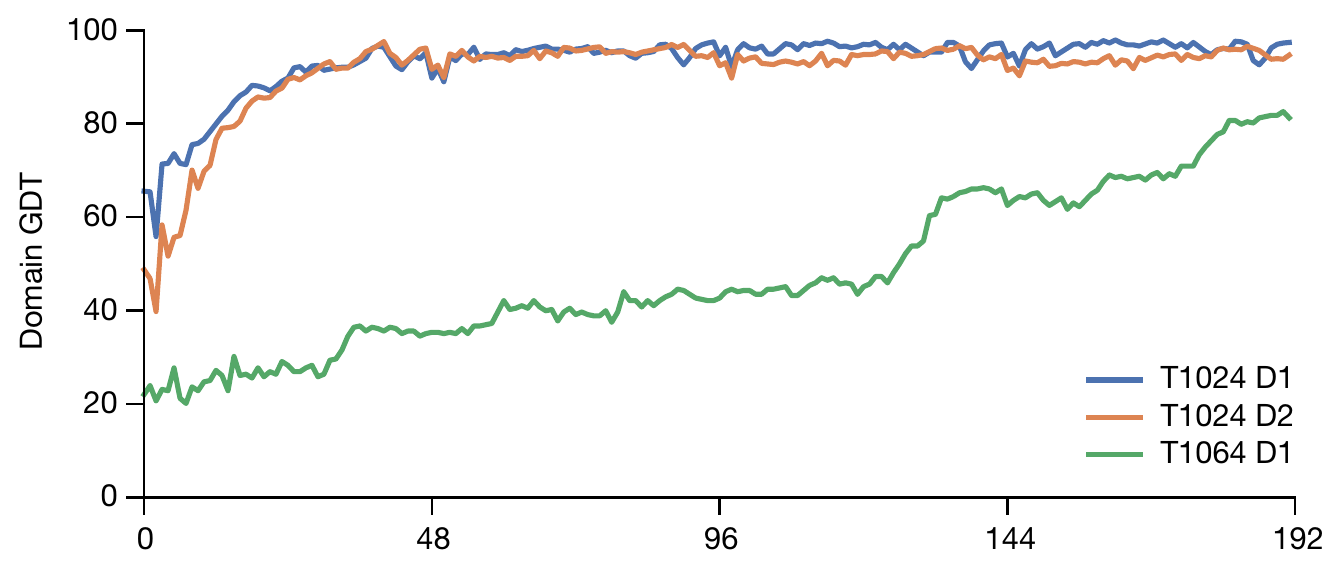
\includegraphics[scale=0.4]{images/af2-iterazioni.png}
	\caption{Traiettoria del valore del GDT sui domini di due target del CASP14 (T1024, composta da due domini e T1064) con 4 iterazioni del modello. Da notare che 48 blocchi dell'Evoformer costituiscono un ciclo di iterazione. I due domini T1024 ottengono la struttura corretta presto, mentre il target T1064 richiede praticamente tutta la profondità della rete per raggiungere una buono struttura finale. Fonte\cite{jumper2021highly}}
	\label{fig:af2-iterazioni}
\end{figure}

\subsection{Evoformer}
L'Evoformer è il primo componente della struttura di AF2 a cambiare le "regole" dei sistemi di predizione classici. Il compito dell'Evoformer è di spremere ogni goccia di informazione dall'MSA, dai template e dalle altre informazioni derivanti dall'analisi di sequenze. Sono decenni che vengono estratte informazioni attraverso analisi coevolutive, ma fino al CASP13 erano perlopiù approcci statistici. Molti gruppi hanno però dimostrato che attraverso l'uso di ResNet profonde non c'era bisogno di una robusta e complicata statistica. AlphaFold2 reinventa completamente questo processo di analisi coevolutiva e la porta ad un livello di utilità molto superiore.

\begin{figure}[!htb]
	\centering
	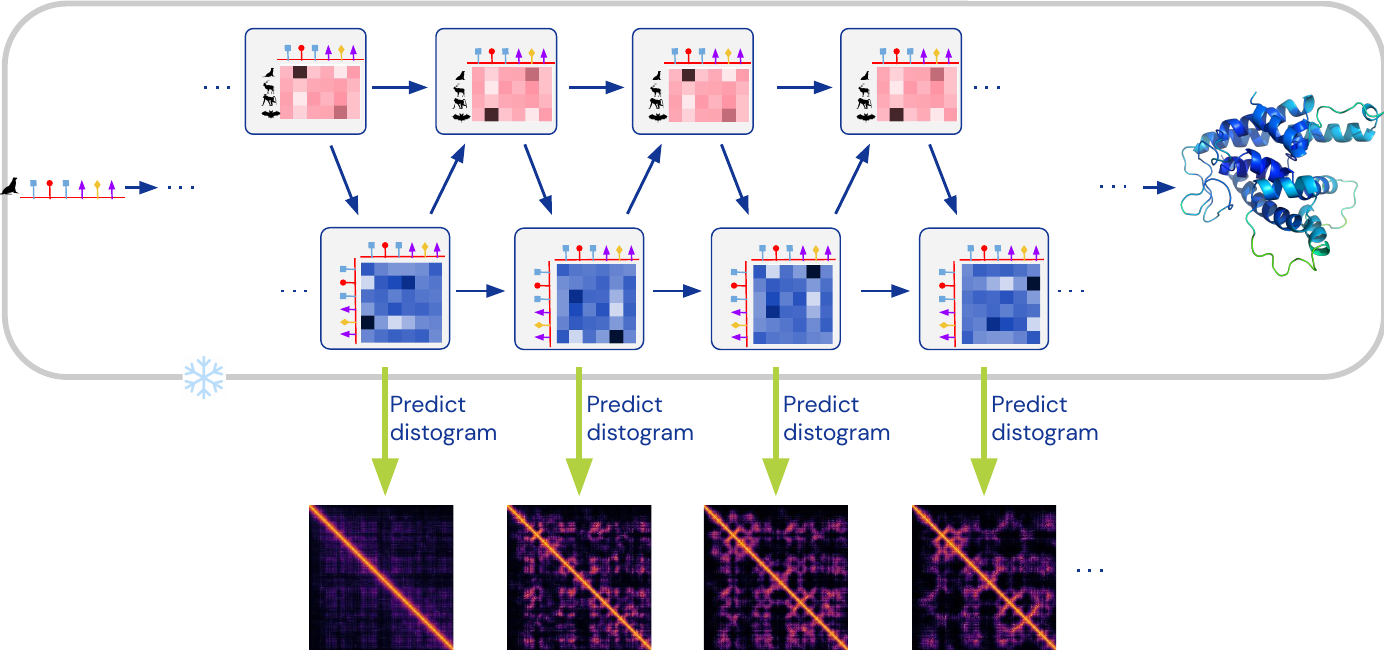
\includegraphics[scale=0.42]{images/evoformer2.png}
	\caption{Rete di AF interrogata sui distogrammi previsti. La previsione dei distogrammi è uno dei principali passi che AF compie per "comprendere" la struttura della proteina. Fonte\cite{AFslide}}
	\label{fig:evoformer-distogram}
\end{figure}

\par L'idea centrale dietro l'Evoformer è che le informazioni fluiscono avanti e indietro attraverso la rete. Prima di AlphaFold 2, la maggior parte dei modelli di deep learning richiedeva un allineamento di sequenze multiple e generava alcune inferenze sulla prossimità geometrica. L'informazione geometrica era quindi un prodotto della rete. Nell'Evoformer, invece, la \textit{pair representation} è sia un prodotto che uno strato intermedio. Ad ogni ciclo, il modello sfrutta l'attuale ipotesi strutturale per migliorare la valutazione dell'allineamento di sequenze multiple, che a sua volta porta a una nuova ipotesi strutturale, e così via. Entrambe le rappresentazioni, sequenza e struttura, si scambiano informazioni finché la rete non raggiunge una solida inferenza.

Il primo passo nella rete è definire gli \textit{embeddings} (incorporamenti) per l'MSA e i template. Gli allineamenti di sequenze multiple sono in ultima istanza sequenze di simboli su un alfabeto finito e quindi un esempio di variabile discreta. Le reti neurali, invece, sono intrinsecamente continue e si basano sulla differenziazione per apprendere dal loro training set. 

\par Un \textit{embedding} è un "trucco" del deep learning che consente la trasformazione di una variabile discreta in uno spazio continuo (\textit{embedded space}) in modo che la rete possa essere addestrata. È un processo molto semplice: c'è solo bisogno di definire uno strato di neuroni che riceve l'input discreto ed emette un vettore continuo. Un \textit{embedding}, più precisamente, è uno spazio di dimensioni relativamente basse in cui è possibile tradurre vettori di dimensioni elevate.  Idealmente, un \textit{embedding} acquisisce parte della semantica dell'input posizionando input semanticamente simili vicini nello spazio di incorporamento.  Un incorporamento può essere appreso e riutilizzato tra i modelli. L'embedding dettagliato che AF2 compie sulle caratteristiche di input può essere osservato in figura \ref{fig:af2-emebddings} \footnote{I dettagli applicativi di ogni variabile e algoritmo sono consultabili nelle informazioni supplementari del paper di AlphaFold: \fullcite{supplementaryjumper2021highly}.}.

\begin{figure}[!htb]
	\centering
	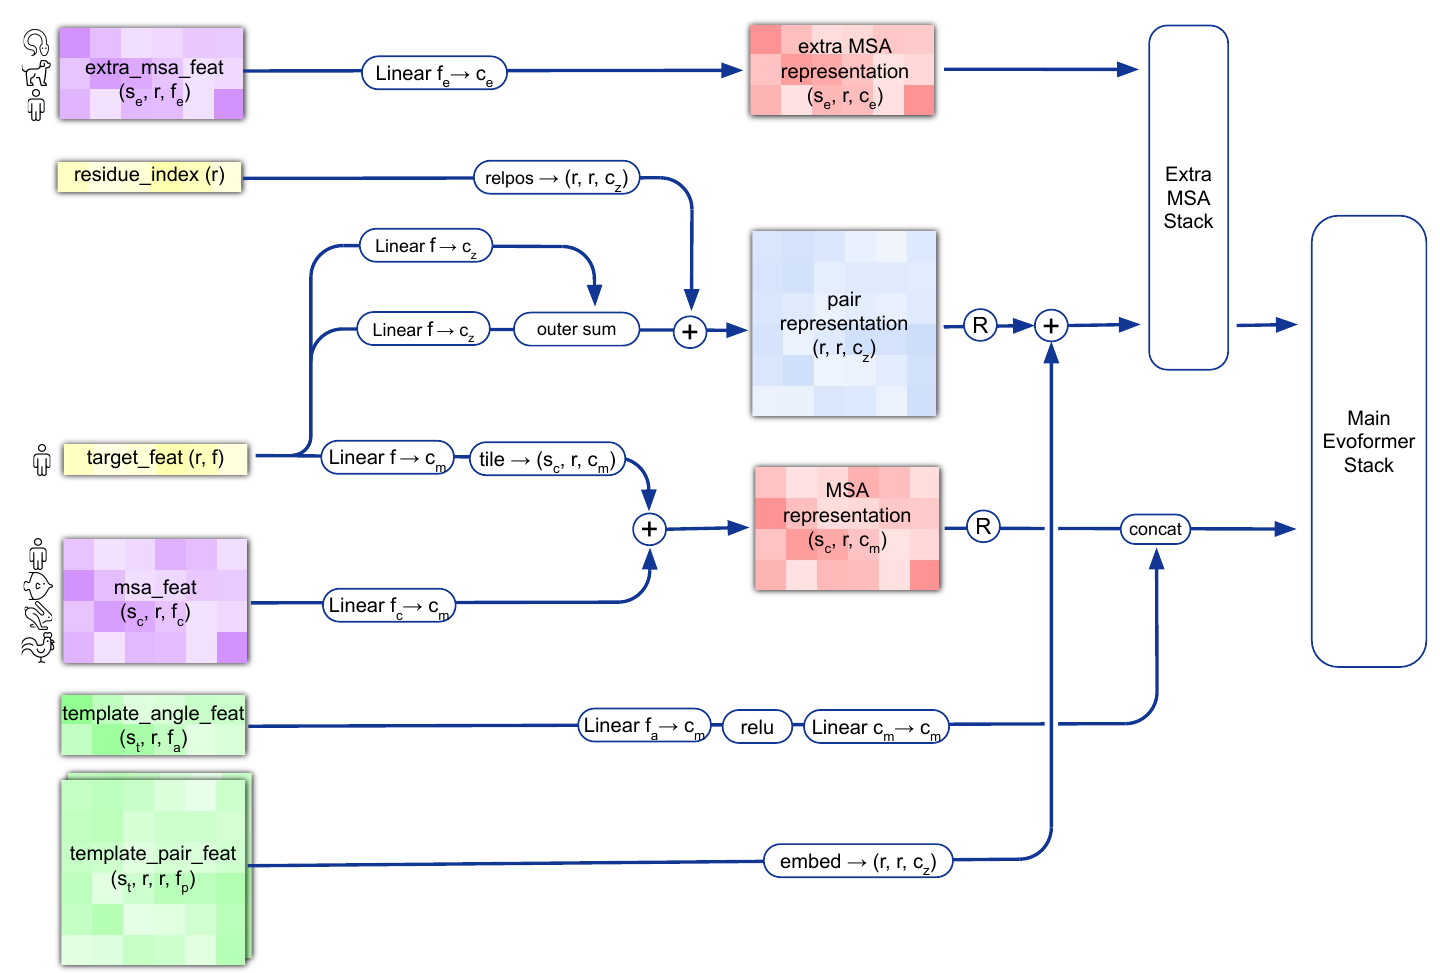
\includegraphics[scale=0.46]{images/af2-input-embeddings.png}
	\caption{Input feature embeddings. Fonte\cite{supplementaryjumper2021highly}}
	\label{fig:af2-emebddings}
\end{figure}

L'architettura dell'Evoformer usa due \textit{transformer}, connessi da un canale di comunicazione tra i due. Ognuno è specializzato in un certo tipo di dati: MSA o interazioni fra coppie di amminoacidi. 

\par L'architettura \textit{transformer} è stata introdotta nel 2017 da un gruppo del Google Brain\supercite{vaswani2017attention} e l'ingrediente chiave 
di tale architettura è chiamata \textit{attenzione}. L'obiettivo dell'\textit{attenzione} è identificare quali parti dell'input sono più importanti per l'obiettivo della rete neurale. I transformer hanno dimostrato empiricamente prestazioni superiori in una varietà di compiti, ad esempio nell'\textit{image captioning} e nel \textit{machine translation}. In quest'utlimo problema aiutano a migliorare il problema del \textit{vanishing gradient}, un ostacolo comune durante l'allenamento. Nei modelli basati su sequenze, possono accelerare significativamente l'addestramento rispetto ai classici modelli di RNN. In particolare, sono alla base della maggior parte dei risultati più clamorosi dell'IA degli ultimi anni: ad esempio, GPT in \textit{GPT-3} sta per "Generative Pre-training Transformer".

\par C'è anche un contro all'uso dei transformer: la costruzione della matrice di attenzione richiede un costo in memoria quadratico. Per questa ragione le Tensor Processing Unit (TPU) introdotte da Google apportano notevoli vantaggi.

\par Il primo transformer, denominabile anche \textit{MSA transformer}, calcola l'attenzione su una matrice molto ampia. Per ridurre quello che altrimenti sarebbe un problema computazionale intrattabile, l'attenzione "fattorizza" in componenti \textit{riga} e \textit{colonna}. Questo processo prende il nome di \textit{axial-attention}. La struttura a livelli consente di calcolare la maggioranza del contesto in parallelo durante la decodifica senza introdurre alcuna ipotesi di indipendenza. In questo contesto, semplificando, la rete calcola prima l'attenzione in orizzontale, consentendo alla rete di identificare quali coppie di amminoacidi sono più correlate; e poi in direzione verticale, determinando quali sequenze sono più informative. 

\par La caratteristica più importane dell'MSA transformer di AF2 è che il meccanismo di attenzione \textit{row-wise} incorpora informazioni dalla \textit{pair representation} come si può vedere in figura \ref{fig:evoformer}, in modo da focalizzarsi sulle coppie di residui che interagiscono fra loro.

\begin{figure}[!htb]
	\centering
	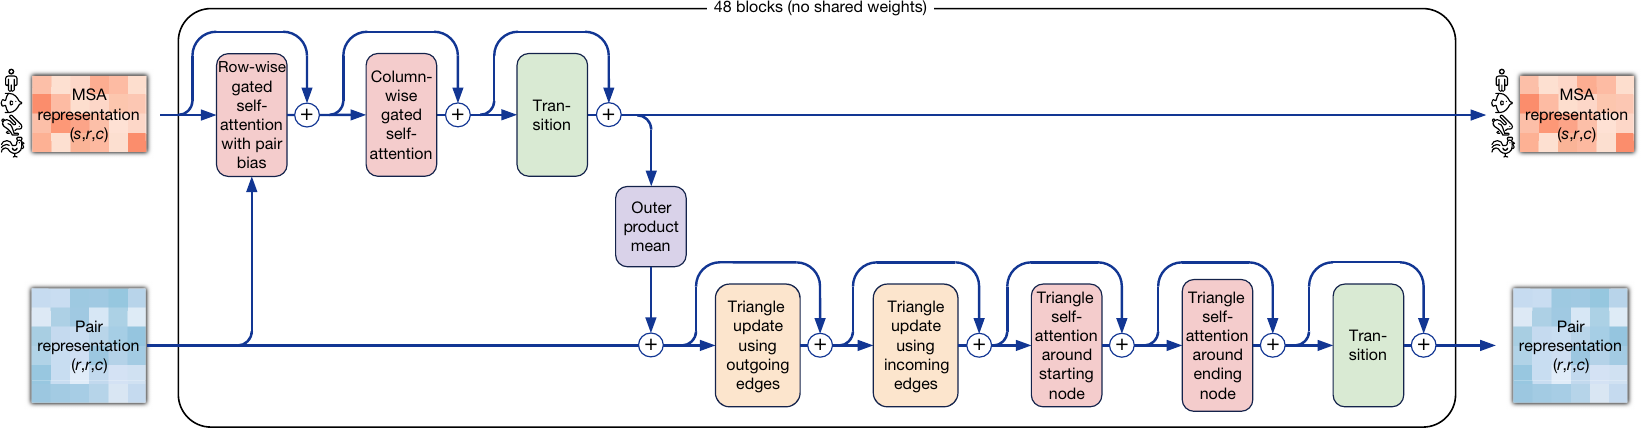
\includegraphics[scale=0.36]{images/evoformer.png}
	\caption{Blocco dell'Evoformer, le frecce indicano il flusso dell'informazione. Fonte\cite{jumper2021highly}}
	\label{fig:evoformer}
\end{figure}

L'altro transformer, denominabile \textit{pair transformer}, si basa su un'impostazione fondamentale: l'attenzione è disposta in termini di triangoli di residui (vedi fig. \ref{fig:triangoli-residui}), con l'obiettivo di sfruttare la disuguaglianza triangolare:

\begin{figure}[!htb]
	\centering
	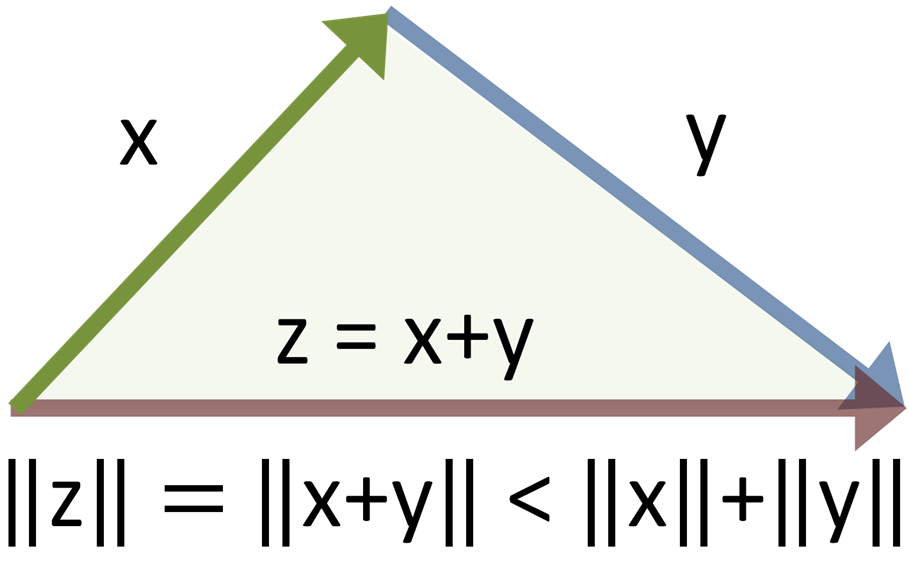
\includegraphics[scale=0.15]{images/disuguaglianza triangolare.PNG}
	\caption{Disuguaglianza triangolare. Fonte\cite{disTriang}}
	\label{fig:}
\end{figure}

Quest'idea permette di superare un problema classico degli approcci basati su DL per il PSP: le distribuzioni di distanze non potevano essere \textit{embedded} nello spazio tridimensionale. 

\begin{figure}[!htb]
	\centering
	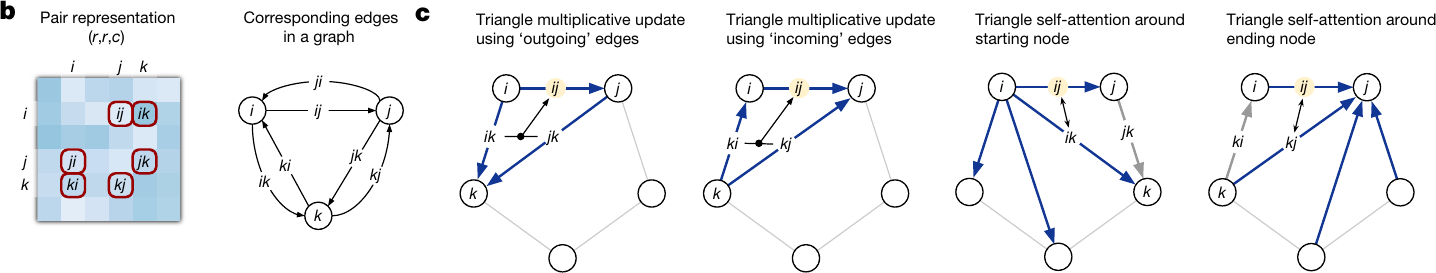
\includegraphics[scale=0.42]{images/triangoli.png}
	\caption{(b) Pair representation interpretata a grafo. (c) Aggiornamenti moltiplicativi ai triangoli di residui e self-attention. I dati nella pair representation sono illustrati come archi direzionati e in ogni diagramma l'arco aggiornata è "ij". Fonte\cite{jumper2021highly}}
	\label{fig:triangoli-residui}
\end{figure}

Dopo un certo numero di iterazioni, 48 nel paper, la rete ha costruito un modello delle interazioni all'interno della proteina. 


\subsection{Structure Module}

In questo modulo viene rappresentata tridimensionalmente la struttura attraverso un ripiegamento \textit{end-to-end} (invece di un metodo a discesa di gradiente). La proteina viene considerata come un \textit{gas residuo}, la backbone è un gas di corpi rigidi 3D. Gli amminoacidi vengono modellati come triangoli, rappresentando i 3 atomi della backbone. 

\par All'inizio i residui vengono tutti piazzati nell'origine (\textit{black hole inizialization}). Ad ogni step del processo iterativo vengono prodotte delle matrici di \textit{affinità} (via matematica per rappresentare traslazioni e rotazioni in una matrice $4\times 4$).

\par Vengono effettuate 8 iterazioni per ridurre le violazioni stereochimiche e raffinare la struttura. Tuttavia anche dopo il processo di raffinamento è possibile che la struttura presenti delle violazioni. Per questa ragione vengono eseguiti dei raffinamenti ulteriori attraverso una discesa di gradiente vincolata dalle coordinate precedentemente calcolate, usando il campo di forza Amber ff99SB con OpenMM.

\begin{figure}[!htb]
	\minipage{0.5\textwidth}
	\centering
	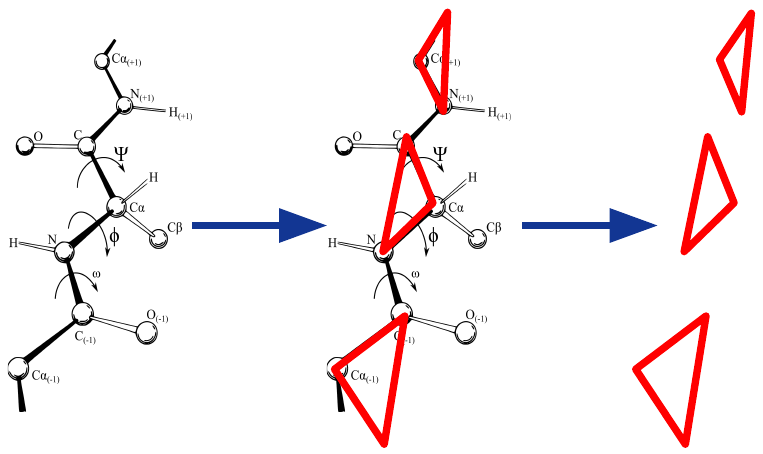
\includegraphics[scale=0.4]{images/gas-residue.png}
	\caption{Rappresentazione come gas residuo. Fonte\cite{AFslide}}
	\label{fig:gas-residuo}
	\endminipage\hfill
	\minipage{0.48\textwidth}
	\centering
	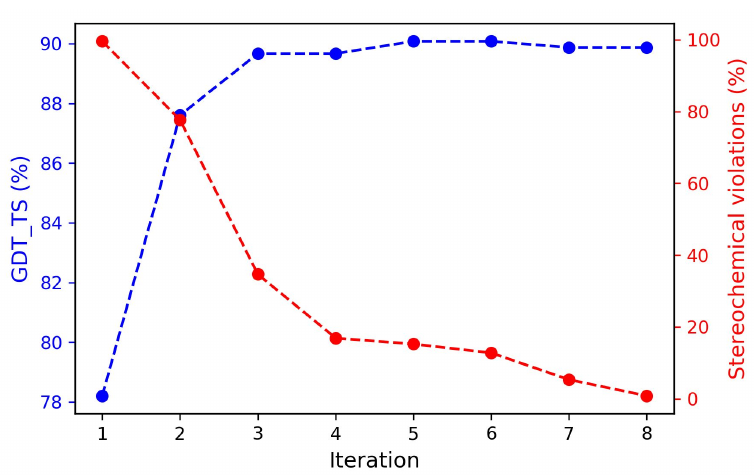
\includegraphics[scale=0.4]{images/struct-module.png}
	\caption{Miglioramento dell'accuratezza e diminuzione delle violazioni stereochimiche attraverso le iterazioni del modulo. Fonte \cite{AFslide}}
	\label{fig:structure-module-iterazioni}
	\endminipage\hfill
\end{figure}

\par I corpi rigidi vengono aggiornati da un'architettura transformer equivariante 3D, che costruisce anche i gruppi laterali (parametrizzati da una lista di angoli  di torsione). Questa è una nuova architettura basata sull'attenzione ideata specificatamente per lavorare con strutture tridimensionali: \textit{Invariant Point Attention} (IPA). Questo meccanismo di attenzione beneficia del fatto di essere invariante rispetto alle traslazioni e alle rotazioni, necessitando così di meno dati.

\begin{figure}[!htb]
	\centering
	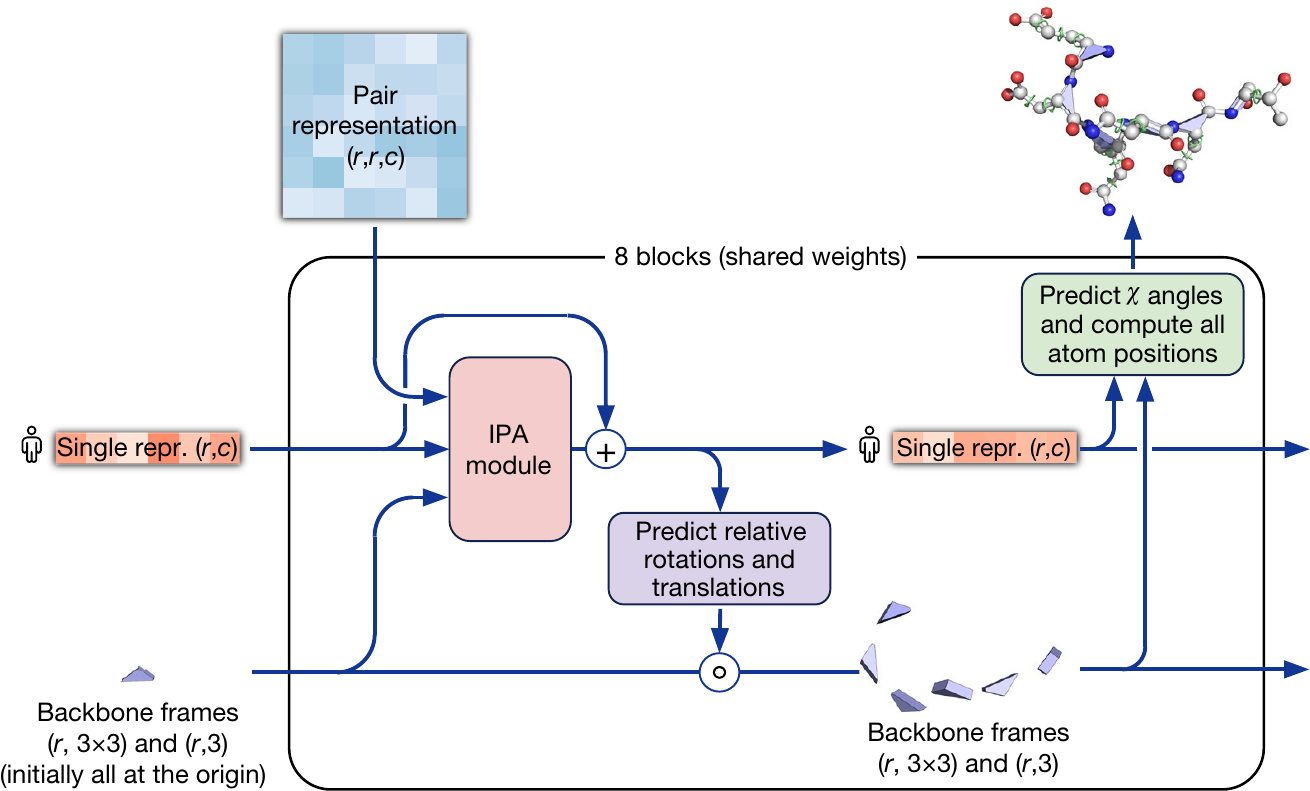
\includegraphics[scale=0.4]{images/structure-module-ipa.png}
	\caption{Structure module compreso IPA. Fonte\cite{jumper2021highly}}
	\label{fig:struct-ipa}
\end{figure}

\par Come rappresentazione iniziale viene usata la prima riga dell'Evoformer (la "single representation" è una copia della prima riga dell'MSA representation, ovvero una sequenza) ed è chiamata $s_{i}$. La \textit{pair representation} influenza le matrici di affinità nelle operazioni di attenzione. Le iterazioni sono 8 perché vi sono 8 strati nel modulo con pesi condivisi. Ogni strato aggiorna la rappresentazione singola astratta ($\{s_{i}\}$) così come la rappresentazione 3D (gas residuo).

\par Uno strato dello structure module è composto da 3 principali operazioni, nelle quali la singola rappresentazione astratta: 

\begin{enumerate}
	\item viene aggiornata dall'Invariant Point Attention (algoritmo 20 riga 6, vedi \ref{fig:alg20}) 
	\item viene aggiornata da un layer di transizione
	\item infine viene mappata su frame di aggiornamenti concreti che sono parti dei frame della backbone
\end{enumerate}

\begin{figure}[!htb]
	\centering
	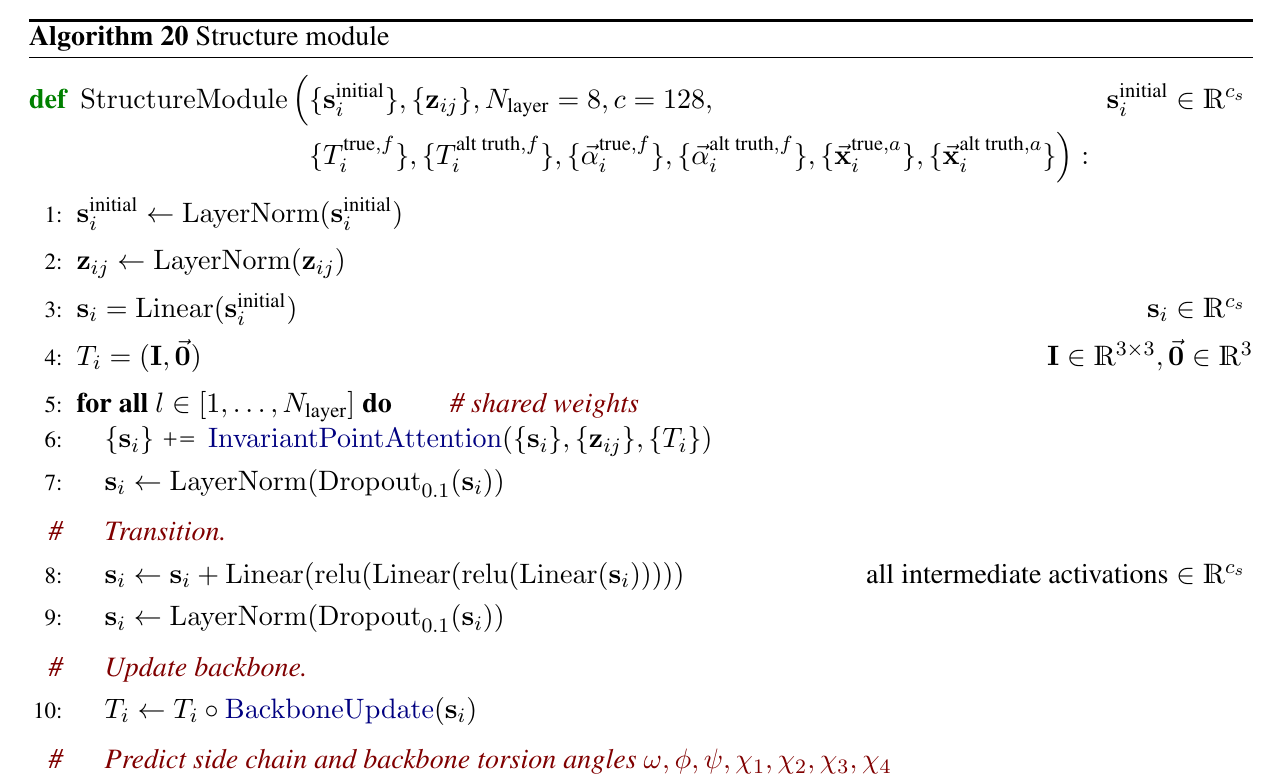
\includegraphics[scale=0.5]{images/alg20.png}
	\caption{Structure Module, prime 10 righe dello pseudocodice. Le righe qui fatte notare sono la 6 a la 10. Fonte\cite{supplementaryjumper2021highly}}
	\label{fig:alg-20}
\end{figure}

L'aggiornamento dei frame della backbone (algoritmo 20 riga 10) avviene tramite la predizione di un \textit{quaternione} per la rotazione e di un vettore per la traslazione. L'utilizzo dei quaternioni è utile perché...

\subsection{Altri dettagli}

La citazione ironica di AlQuraishi raccoglie forse al meglio le scelte strutturali in AlphaFold:

\say{\textit{For AlphaFold2, the apparent answer that DeepMind gave to the question of what they should do
		is... yes. Self-supervision? Yes. Self-distillation? Yes. New loss function? Yes. 3D refinement? Yes.
		Recycling after refinement? Yes. Refinement after recycling? Yes. Templates? Yes. Full MSAs? Yes.
		Tied-weights? Yes. Non-tied weights? Yes. Attention over nodes? Yes. Attention over edges? Yes.
		Attention over coordinates? Yes. The answer, to all the questions, is yes! And this clearly paid off.}}\footnote{\fullcite{moalqAF2}}\\

\subsubsection{Loss}

La rete è allenata end-to-end con gradienti provenienti dalla funzione di \textit{loss} (funzione obiettivo/di costo) FAPE (Frame Aligned Point Error) e da altre loss ausiliarie:

\begin{figure}[!htb]
	\centering
	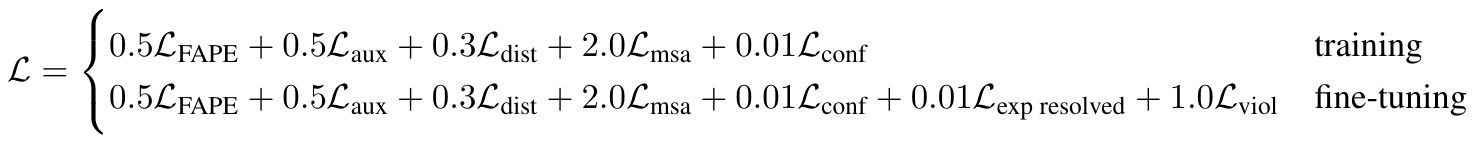
\includegraphics[scale=0.4]{images/loss.png}
	\label{fig:loss}
\end{figure}

dove per \textit{aux} si intende "auxiliary loss", per \textit{dist} "cross-entropy loss for distogram prediction", per \textit{msa} "cross-entropy loss for masked MSA prediction", per \textit{conf} "model confidence loss". La loss totale nella fasi di inferenza comprende anche le loss \textit{exp resolved} che sta per "experimentally resolved loss" e \textit{viol} che sta per "violation loss".\\

\par La loss finale in AF2 è quindi una somma pesata di loss ausiliarie multiple, che non sono necessariamente correlate con le performance ma possono fornire informazioni aggiuntive. Non viene calcolata la loss solo dell'ultima struttura finale dopo le iterazioni, ma viene calcolata per ogni iterazione. È presente anche una \textit{distogram loss} dove la struttura predetta è usata per generare un distogramma (matrice 2D di intervalli di probabilità di distanze) da confrontare con la "realtà di base" (\textit{ground truth}, ovvero dalle strutture PDB con più accuratezza).

\par Un'altra loss interessante è l'\textit{MSA masking}. Ad ogni step al modello viene fornita una MSA con alcuni simboli "mascherati" e gli viene chiesto di predirli. È un modo per crearsi da sé un apprendimento supervisionato, come reso popolare da BERT, ed è usato sia nella fase di training che di inferenza.\\

\par Un altro dettaglio è la \textit{self-distillation}. L'architettura di AF2 è in grado di allenarsi con grande accuratezza solamente tramite il \textit{supervised learning} sui dati provenienti dal PDB. È stato però trovato il modo di aumentare l'accuratezza usando un approccio simile al \textit{noisy student self-distillation}\supercite{xie2020self}. In questa procedura viene usata una rete già addestrata per predire la struttura di circa 350.000 sequenze diverse da Uniclust30; viene poi creato un nuovo set di dati di strutture previste, filtrate in un sottoinsieme ad alta confidenza. Viene poi addestrata di nuovo la stessa architettura da zero utilizzando una combinazione di dati dal PDB e da questo nuovo set di dati di strutture previste come \textit{training data}. Questa procedura ha lo scopo di fare un uso efficace delle sequenze non etichettate e aumenta considerevolmente l'accuratezza della rete risultante (vedi fig. \ref{fig:ablazione1}). 

\subsubsection{Training}

AF2 viene addestrato in un modo apparentemente strano: non su intere proteine, ma su frammenti di alcune, ciò che il team di AF2 chiama \textit{crops}. Di solito i \textit{crops} sono composti da un paio di centinaia di residui, quindi solo una frazione di grandi proteine.

\par Sorprendentemente, mentre AF2 è principalmente addestrato su frammenti fino a 256 residui (successivamente perfezionato a 384), può prevedere strutture proteiche con ben oltre 2.000 residui. Sembrerebbe un task quasi impossibile in apparenza: come si è già visto il contesto globale è fondamentale nel protein folding, due sottosequenze di amminoacidi uguali, in due differenti proteine, non si ripiegano allo stesso modo in genere. Ci sono però due fattori che consentono ad AF2 di affrontare la sensibilità al contesto:

\begin{itemize}
	\item AF2 lavora con MSA o pattern coevolutivi, che codificano informazioni a prescindere dalla separazione nella catena
	\item durante la fase di inferenza AF2 usa l'intera sequenza
\end{itemize}

Quest'idea di disaccoppiare cose generalmente accoppiate stride con i modelli comuni nel ML dove le fasi di training e inferenza vengono tenute molto simili, basandosi sull'idea che più i due processi sono simili migliore sarà la predizione finale. In questo caso nella fase di allenamento è importante che il modello acquisisca informazioni con aggiornamenti dei gradienti. Nonostante AF2 non sia l'unica architettura ad aver adottato questa strategia (es. modelli generativi) essa è un’implementazione robusta dell’idea. È possibile che sia stata progettata in questo modo solamente per efficienza di memoria (sarebbe impossibile allenare su proteine intere una struttura della grandezza di AF2) ma tale scelta si è rivelata una buona idea anche dal punto di vista biofisico.

\subsection{Analisi via ablazione}

Per \textit{ablazione} si intende la valutazione delle prestazioni del sistema rimuovendo uno o più componenti non essenziali o combinazioni di questi. Questo studio è interessante perché può rivelare l'importanza e l'efficacia di determinati componenti. Non si possono trarre conclusioni generali ma si può ipotizzare quali siano le parti più importanti per generare predizioni di qualità.

\par Il modello \textit{baseline} è il modello come descritto nel paper ad eccezione del meccanismo di \textit{self-distillation}. Viene utilizzato come base per i confronti in questi studi di ablazione. 

\begin{figure}[!htb]
	\centering
	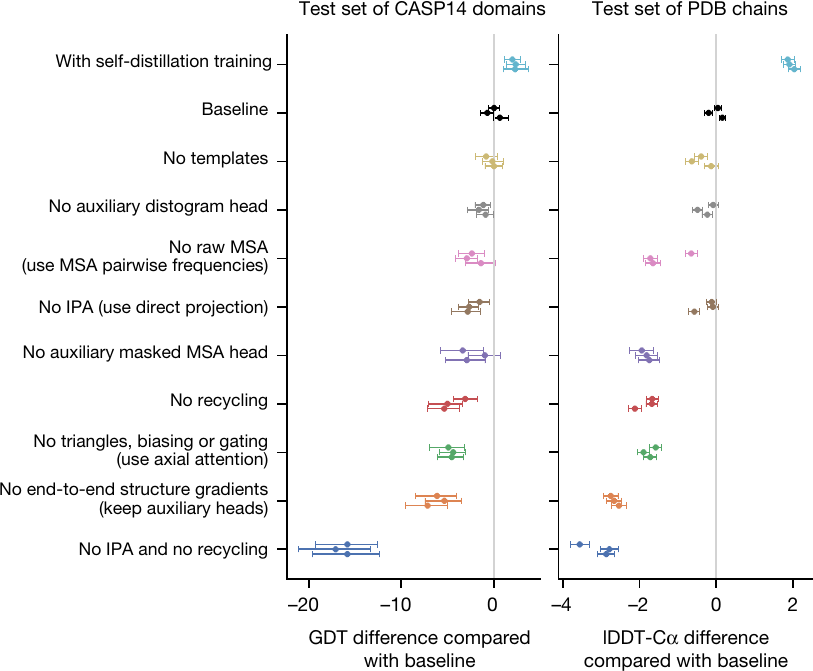
\includegraphics[scale=0.6]{images/ablazione.png}
	\caption{Risultati di ablazione di vari componenti su due target set: insieme di domini del CASP14 (n=87), PDB test set di catene con copertura di identità minore del 30\% (n=2.261). Fonte: \cite{jumper2021highly}}
	\label{fig:ablazione1}
\end{figure}

\begin{figure}[!htb]
	\centering
	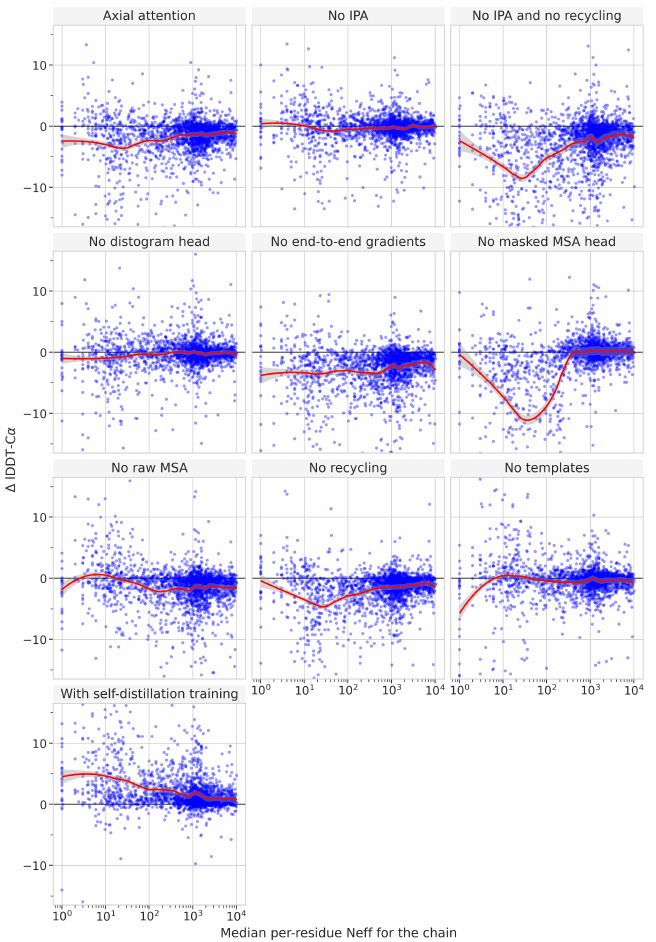
\includegraphics[scale=0.7]{images/ablazione2.png}
	\caption{Accuratezza in esperimenti di ablazione relativi alla baseline per differenti valori di profondità dell'MSA su recenti insiemi di proteine dal PDB, filtrati da una copertura da template <30\%(n=2.261). Fonte \cite{supplementaryjumper2021highly}}
	\label{fig:ablazione-2}
\end{figure}

\par Ad esempio una caratteristica che può saltare all'occhio è l'apparente bassa influenza dell'IPA, nonostante sia una struttura complessa a cui il team  ha dedicato molto tempo. Senza IPA lo structure module si basa solo sulla rappresentazione 1D per la generazione della struttura. Il punto fondamentale è che le performance non cambiano molto se si toglie l'IPA, a patto che il recycling venga lasciato. Quando entrambi sono tolti si può vedere (fig. \ref{fig:ablazione1}) che le performance calino nettamente. Tuttavia se viene rimosso il recycling ma lasciata l'IPA le performance non subiscono grandi differenze, ed è importante notare ciò in quanto mostra che l'IPA è una struttura incredibilmente efficiente rispetto all'evoformer: con il recycling vengono triplicati i 48 blocchi dell'evoformer mentre l'IPA è composta di soli 8 layer.

\par In figura \ref{fig:ablazione-2} si può notare l'accuratezza di AF2 quando vengono tolti alcuni componenti, su sequenze con MSA poco profonde. Un dettaglio che risalta è l'importanza della funzione di loss relativa al mascheramento dell'MSA e di mantenere almeno uno fra IPA e recycling. Grazie a questi accorgimenti AF2 riesce ad avere ottima accuratezza anche quando l'MSA è poco profonda ed è forse proprio questo uno dei più grandi raggiungimenti di DeepMind.


\subsection{Differenze con AF1}

AlphaFold1 lavora sulla premessa che data una sequenza proteica, è possibile costruire un potenziale appreso e specifico per le proteine, addestrando una rete neurale profonda (DNN) per fare previsioni accurate sulla struttura e per prevedere la struttura stessa riducendo al minimo il potenziale mediante discesa del gradiente.

\par Le caratteristiche usate nella DNN sono caratteristiche MSA generate eseguendo HHblits e PSI-BLAST su database di sequenze. La DNN prevede gli angoli di torsione della backbone e la distanza a coppie tra i residui. Quindi, la distanza prevista e le distribuzioni di probabilità di torsione insieme alle interazioni di  van der Walls vengono combinate per formare un potenziale specifico della proteina. Infine, viene eseguita la discesa del gradiente sul potenziale specifico della proteina per ottenere il modello proteico finale. 

\par I dati di addestramento per il modello di AF1 vengono estratti dai domini PDB e più specificamente CATH in cui sono state utilizzate 29.427 proteine ​​per l'addestramento e 1820 proteine ​​vengono utilizzate per i test. Le buone prestazioni di AlphaFold sono attribuite all'accuratezza delle previsioni di distanza\supercite{pakhrin2021deep}.

\par L'idea di ridurre al minimo il potenziale mediante la discesa del gradiente piuttosto che utilizzare l'assemblaggio dei frammenti e la successiva raffinazione del modello è piuttosto nuova.

\par La prima macro differenza tra i due sistemi è che AlphaFold 1 (AF1) conteneva moduli addestrati separatamente, mentre AlphaFold2 lo ha sostituito con un sistema di sottoreti accoppiate insieme in un sistema di deep learning end-to-end formato come un'unica struttura integrata.

\begin{figure}[!htb]
	\centering
	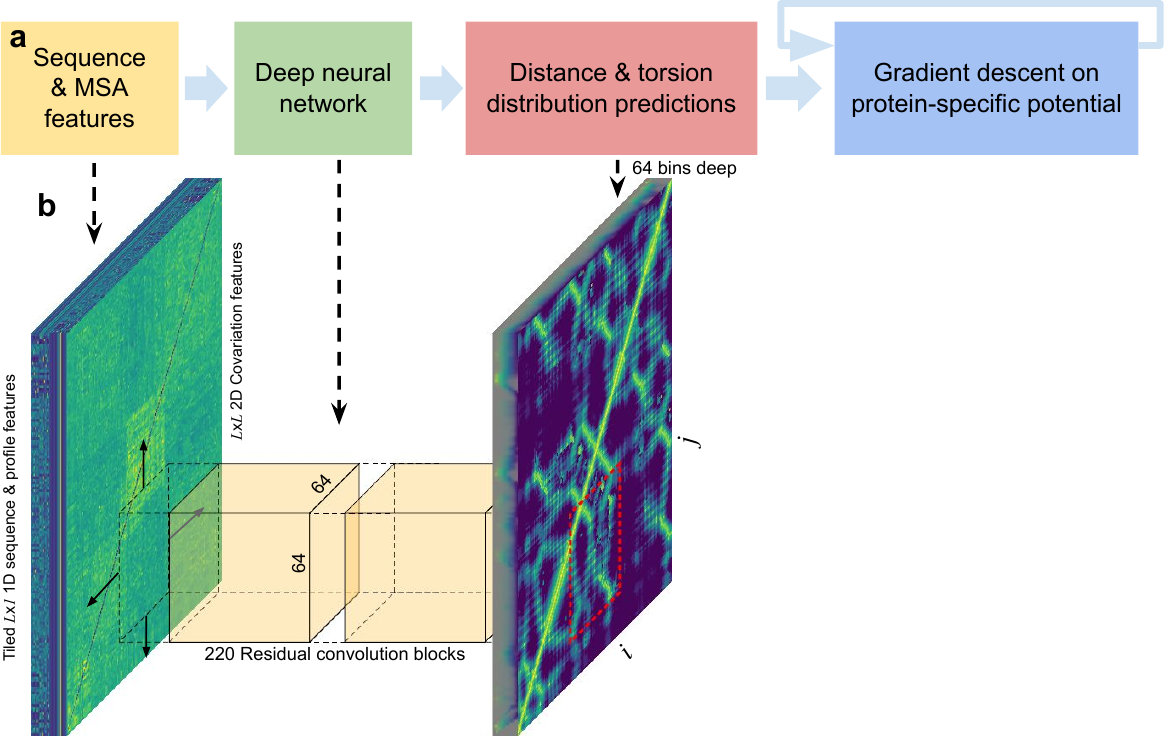
\includegraphics[scale=0.5]{images/af1.png}
	\caption{ Struttura di AF1. Length L = 155. (a) Step della predizione della struttura. (b) La rete neurale predice l'intero distogramma L×L basato su caratteristiche dell'MSA, accumulando predizioni separate per regioni di residui 64×64. Fonte\cite{senior2020improved}}
	\label{fig:af1}
\end{figure}

\par Rispetto alla prima iterazione di AlphaFold apparsa nel CASP13, guidata dalla previsione della \textit{distance map }basata su CNN, uno dei principali nuovi sviluppi di AlphaFold2 è l'architettura della rete neurale basata sull'\textit{attenzione} che interviene arbitrariamente sull'intera MSA. 

\par Inoltre, invece di utilizzare l'ottimizzazione della discesa del gradiente per costruire modelli basati sui vincoli di distanza previsti, come ha fatto AlphaFold in CASP13, AlphaFold2 utilizza un sistema di addestramento completo end-to-end dalla sequenza ai modelli di struttura, utilizzando il raffinamento strutturale iterativo basato sulla stima dell'errore locale. AF2 sostituisce le tradizionali simulazioni di ripiegamento con un modulo strutturale composto da reti neurali di transformer equivarianti 3D, che trattano ciascun amminoacido come un gas di corpi rigidi 3D e costruiscono direttamente la backbone proteica e le catene laterali.

\section{DeepMind}

{
	AlphaFold è un sistema di \textit{Artificial Intelligence }(AI) sviluppato da DeepMind che, come già visto, realizza predizioni allo stato dell'arte sulla struttura delle proteine basandosi sulle loro sequenze amminoacidiche.
	
	\par DeepMind è un'azienda inglese di Intelligenza Artificiale sussidiaria di Alphabet Inc.\footnote{In altre parole DeepMind è una società controllata: Alphabet Inc. detiene la maggioranza dei voti nell'assemblea ordinaria o un'influenza dominante sull'amministrazione.}. La missione a lungo termine di AlphaFold è avanzare il progresso scientifico risolvendo problemi scientifici fondamentali attraverso l'uso di sistemi di AI.
	
	\par DeepMind è stata fondata nel 2010 da Demis Hassabis, Shane Legg e Mustafa Suleyman. La società ha sede a Londra con centri di ricerca in Canada, Francia e Stati Uniti \supercite{deepMindWiki}.
	
	\par Può risultare interessante osservare la correlazione fra i primi lavori di DeepMind e la vita di Demis Hassabis, una vita ricca di sfaccettature: bambino prodigio nel gioco degli scacchi, programmatore di videogiochi (dai 17 anni) passando per una laurea in \textit{Computer Science}, alla fondazione del proprio studio videoludico (Elixir Studios) per poi ritornare nel mondo accademico per ottenere il suo PhD in neuroscienze cognitive nel 2009, campo nel quale ha coautorato numerosi articoli influenti su memoria e amnesia (es. rappresentazione della memoria episodica tramite \textit{scene construction} \supercite{Hassabis2007Jul}) \supercite{hassabisWiki}. Per arrivare infine a fondare DeepMind e la nuovissima società Isomorphic Labs, sempre sussidiaria di Alphabet Inc. che si pone come obiettivo quello di reimmaginare il processo di \textit{drug discovery} con un approccio basato principalmente sull'AI.
	
	\par DeepMind iniziò infatti a focalizzarsi sull'insegnare ad un sistema di AI come giocare a vecchi videogiochi anni '70,'80 (es. Pong, Breakout, Space Invaders), per poi passare al gioco del Go, al protein folding e recentemente alla programmazione competitiva automatizzata \supercite{competitiveProgrDeepMind}.
	DeepMind è stata acquistata da Google nel 2014 per 500 milioni di dollari \supercite{Guardian2014}.
	
	\subsubsection{Etica}
	Dopo l'acquisizione di Google l'azienda ha stabilito un'\textit{AI ethics board}. DeepMind è uno dei membri fondatori di \textit{Partnership on AI} insieme ad Amazon, Google, Facebook, IBM e Microsoft, un'organizzazione dedicata all'interfaccia società-AI \supercite{partnershiponai}.
	
	\par DeepMind ha anche aperto una nuova unità denominata DeepMind Ethics and Society e si è concentrata sulle questioni etiche e sociali sollevate dall'intelligenza artificiale avendo come consulente il famoso filosofo Nick Bostrom. Nell'ottobre 2017, DeepMind ha lanciato un nuovo gruppo di ricerca per studiare l'etica dell'IA.
	
	\subsubsection{Alphabet}
	Alphabet è un'azienda statunitense fondata nel 2015 dagli stessi fondatori di Google (Larry Page e Sergey Brin) come \textit{holding} a cui fa capo Google LLC e altre società sussidiarie: oltre a DeepMind vi sono Calico, CapitalG, Waymo, Wing, Intrinsic, Nest Labs, Sidewalk Labs, Isomorphic Labs, ecc.\\ 
	Da dicembre 2019 il CEO di Alphabet è Sundar Pichai \supercite{cnbc}.
	La fondazione di Alphabet a partire da Google è stata una scelta finalizzata a rendere più trasparenti le attività inerenti a Google e concedere una maggiore autonomia alle società del gruppo che operano in settori diversi da quello dei servizi internet.
}

\clearpage














